\documentclass[14pt, a4paper]{extarticle}
\usepackage{amsmath}
\usepackage{amssymb}
\usepackage{mathtools}
\usepackage{mathtext}
\usepackage[T1, T2A]{fontenc}
\usepackage[utf8]{inputenc}
\usepackage[english, russian]{babel}
\usepackage{cmap}
\usepackage{fancyhdr}
\usepackage[pdftex]{graphicx}
\usepackage{gensymb}
\usepackage{floatrow}
\usepackage{titlesec}
\usepackage{lastpage}
\usepackage{float}
\usepackage{gensymb}
\usepackage{booktabs}
\usepackage{mathrsfs}
\usepackage{floatflt}
\usepackage{wrapfig}
\usepackage{caption}
\usepackage{ upgreek }

\graphicspath{{pictures/}}
\DeclareGraphicsExtensions{.pdf,.png,.jpg}
\newtheorem{task}{Задача}
\begin{document}
\selectlanguage{russian}


\begin{titlepage}
\begin{center}

\textsc{\LARGE Московский\\[-0.2cm]Физико-Технический Институт\\[0.1cm]\large (национальный исследовательский университет)}\\[1.5cm] 


\includegraphics[width=0.3\textwidth]{logo}

\textsc{\Large Лабораторная работа 5.2.2: \\ }

% Title
\HRule \\[0.4cm]
{ \LARGE \bfseries Изучение спектров атома водорода и молекулы йода }

\HRule \\[1.5cm]

% Author and supervisor
\noindent
\begin{minipage}{0.4\textwidth}
\begin{flushleft} \large
\end{flushleft}
\end{minipage}%
\begin{minipage}{0.4\textwidth}
\begin{flushright} \large
\end{flushright}
\end{minipage}

\large{\begin{flushright}
\vfill
\textbf{Выполнил}:\\
\textbf{Маслюк Руслан\\}
\textbf{группа Б05-871}
\end{flushright}}

{\large \today}\\

\end{center}
\end{titlepage}


\section{Цель}
\label{sec:цель}
Изучить спектральные закономерности в оптических спектрах водорода(А) и йода(Б). По результатам вычислим постоянные Ридберга для водорода и йода, их потенциалы ионизации, изотопические сдвиги ланий.
\section{Вступление}
\subsection{Оборудование} % (fold)
\label{sec:оборудование}
		
Для измерения длин волн спектральных линий в работе используется стеклянно-призменный монохроматор-спектрометр УМ-2 (универсальный монохроматор), предназначенный для спектральных исследований в диапазоне от 0,38 до 1,00 мкм\\
Основные элементы монохроматора представлены на рис. 2. \\
1. Входная щель 1, снабженная микрометрическим винтом 9, который позволяет открывать щель на нужную ширину(в диапазоне 0,01-4 мм).\\ 2. Коллиматорный об ектив 2, снабженный микрометрическим винтом 8. Винт позволяет смещать объектив относительно щели при фокусировке спектральных линий различных цветов.\\
3. Сложная спектральная призма 3, установленная на поворотном столике 6. Призма 3 состоит из трех склеенных призм П1, П2 и П3. Первые две призмы с преломляющими углами $30\degree$ изготовлены из тяжелого флинта, обладающего большой дисперсией. Промежуточная призма П3 сделана из крона. Лучи отражаются от ее гипотенузной грани и поворачиваются на $90\degree$. Благодаря такому устройству, дисперсия призм П1 и П2 складываются. 
\\ 4. Поворотный столик 6, вращающийся вокруг вертикальной оси при помощи микрометрического винта 7 с отсчетным барабаном. На барабан нанесена винтовая дорожка с градусными делениями. вдоль дорожки скользитуказатель барабана. При вращении барабана призма поворачивается, и в центре поля зрения появляются различные участки спектра. 
\\5.  Зрительная труба, состоящая из объектива 4 и окуляра 5. 
\\
6. Массивный корпус 11, предохраняющий прибор от повреждений и за-грязнений.
\\7. Оптическая скамья, на которой могут перемещаться рейтеры с источником света и конденсором К, служащим для концентрации света на входнойщели. Входная щель спектрометра, конденсор и источник должны быть наодной высоте. Проходящий через входную щель световой пучок хорошо за-полняет конденсор и призму, если выполнено соотношение $\frac{D_k}{b} = \frac{D_2}{f_2} = \frac{1}{6}$, где $D_k$ - диаметр конденсора, $b$ - расстояние от конденсора до входнойщели, $D_2$ и $f_2$ - диаметр и фокусное расстояние коллиматорного объектива 2. Изображение удобно наблюдать на колпачке с крестиком (таким колпачком прикрывают щель при юстировке системы).\\ 
\\8. Пульт управления (на рис. 2 не показан), служащий для питания источников света и осветительной системы спектрометра.


% section оборудование (end)
\section{Теория} % (fold)
\label{sec:теория}

\ Атом водорода является простейшей атомной системой; для него уравнение Шредингера может быть решено точно. Поэтому спектр атома водорода является предметом тщательного экспериментального и теоритического исследования.\\
\ Объяснение структуры спектра излучения атомов требует знания схемы атомных энергетических уровней, что, в свою очередь, требует решения задачи о движении электронав эффективном поле атома. Для атома водорода в водородаподобных(одноэлектронных) атомов определение энергетических уровней значительно упрощается, т.к. квантово-механическая задача об относительном движении электрона (заряд $-e, \textnormal{масса} m_e$) и ядра (заряд $Z_e$, масса $M$) сводится к задаче о движении частицы с эффективной массой $\mu = m_eM/(m_e+M)$ в кулоновской поле $Ze^2/r.$ Однако даже для водородоподобного атома это решение не является простым.\\
\ Длины волн спектральных линий водородоподобного атома описываются формулой
\begin{equation}
	\frac{1}{\lambda_{mn}} = RZ^2(\frac{1}{n^2} -\frac{1}{m^2}),
\end{equation}
где $R$ - константа, называемая постоянной Ридберга, а $m$ и $n$ - целые числа.\\
\ Формула (1) - обобщенная формула Бальмера.
\ Для объяснения спектра атома водорода Нильс Бор в 1913г. предложил теорию атома, в основу которой положил 3 постулата:
\begin{enumerate}
	\item из всех возможных с точки зрения классической физики орбит в атоме осуществляются только некоторые стационарные орбиты, при движени по которым, вопреки представлениям классической электродинамики, электрон не излучает энергии;
	\item Из всех возможных орбит в атоме осуществляются только те, для которых момент количества движения равен целому кратному величины постоянной Планка  $\hbar = h/(2\pi)$, т.е.
	\begin{equation}
		L = n\hbar
	\end{equation}
	\item Излучение или поглощение энергии проиходит при переходе атома из одного стационарного состояния с другое, а частота излучаемого (поглощаемого) света связана с разностью энергий атома в стационарных состояниях соотношением
	\begin{equation}
		h\upnu = E_2-E_1,
	\end{equation}
	где $\upnu$ - частота излучаемой линии.  
\end{enumerate}

\ Использование этих постулатов с учетом кулоновского взаимодействия между ядром и электроном позволяет легко определить возможные энергетические состояния водородоподобногоатома. Если считать ядро неподвижным, то эти энергетические определяются выражением
\begin{equation}
 	E_n = -\frac{2\pi^2m_e e^4Z^2}{h^2}\frac{1}{n^2}	
 \end{equation} 
 \begin{wrapfigure}{r}{0.52\linewidth}
 	\centering
 	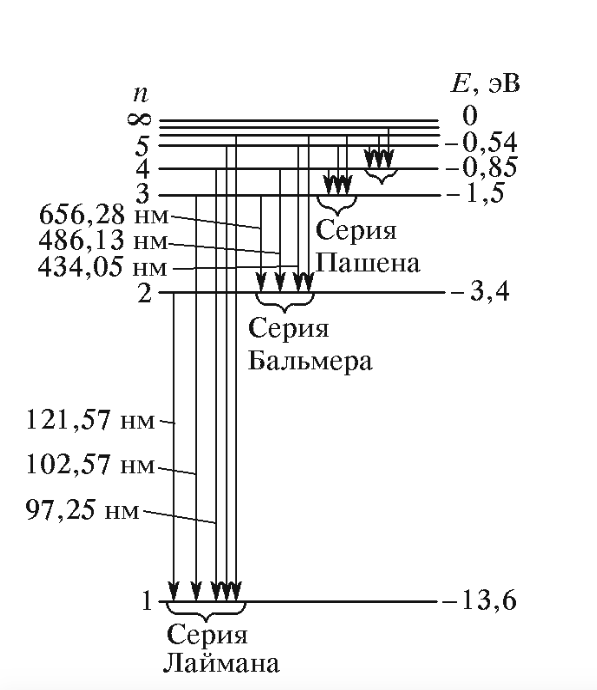
\includegraphics[width = 0.5\linewidth]{Energy_levels}
 	\caption{Уровни Энергии атома водорода и образование спектральных серий}
 \end{wrapfigure}
 \ В свою очередь, знание энергетических состояний атома позволяет в соответствии с формулой (4) определить возможные частоты его излучения и объяснить наблюдаемые спектральные закономерности (Рис.1). \\
 \ Из Рис.1. видно, что линии в спектре водорода можно расположить по сериям ($n = const, m - \textnormal{любое} от n+1 \textnormal{до} \infty$).
 \ В данной работе изучается серия Бальмера, линии которой лежат в видимой области, и изотропический сдвиг между линиямиводорода и йода. Для серии Бальмера n = 2, величина m для первых 4 линий этой серии принимает значение 3,4,5,6. эти линии обозначаются символами $H_\alpha, H_\beta,H_\gamma, H_\delta$.
 \ Рассмотрим, как можно оценить энергии основного и возбужденного состояний водородоподобного атома. Потенциальная энергия электрона равнакулоновской энергииэлектрона в поле ядра с зарядом $Ze$. Так как электрон локализован в области r(орбита), то по соотношению неопределенностей его импульс $p\simeq \hbar/r$ и, следовательно полная энергия определяется вырашением 
 \begin{equation}
  	-\frac{Ze^2}{r}+\frac{\hbar^2}{2m_er^2}.
 \end{equation} 
 Условия минимального значения энергии:
 \begin{equation}
 	\frac{Ze^2}{r^2} - \frac{\hbar^2}{m_er^3} = 0, 
 \end{equation} или
 \begin{equation}
 	r_\textnormal{Б} = \frac{\hbar^2}{Zm_ee^2}.
 \end{equation}
 Мы получили значение боровского радиуса (первая орбита) для электрона в поле ядра с зарядом Z. Энергию получим подставляя (7) в (5):
 \begin{equation}
 	E = -\frac{m_ee^4}{2\hbar^2}Z^2 = -RZ^2.
 \end{equation}
 Аналогично находятся энергии возбужденных состояний. дискретные значения энергии электрона в атоме получаются из того, что на длине орбиты, по которойдвижется электрон, должно укладываться целое число волн де Бройля.
 Тогда для n-го радиуса получим: 
 \begin{equation}
 	p \simeq \frac{\hbar}{\lambda} = \frac{n\hbar}{r} 	
 \end{equation} 
 \begin{equation}
 	T\simeq \frac{n^2\hbar^2}{2m_er^2}
 \end{equation}
 \begin{equation}
 	r_n = \frac{n^2\hbar^2}{Zm_ee^2},
 \end{equation}
 \begin{equation}
 	E_n = -\frac{m_eZ^2e^4}{2\hbar^2}\frac{1}{n^2} = -R\frac{Z^2}{n^2}
 \end{equation}

% section теория (end)
 \section{Ход работы} % (fold)
 \label{sec:ход_работы}
 
 \subsection*{А) Измерение длин волн спектральных линий водорода}
 \begin{enumerate}
 	\item Проградуируем спектрометр по спектрам ртути и неона и построим график:
 	\clearpage
 	\begin{figure}[h!]
 		\centering
 		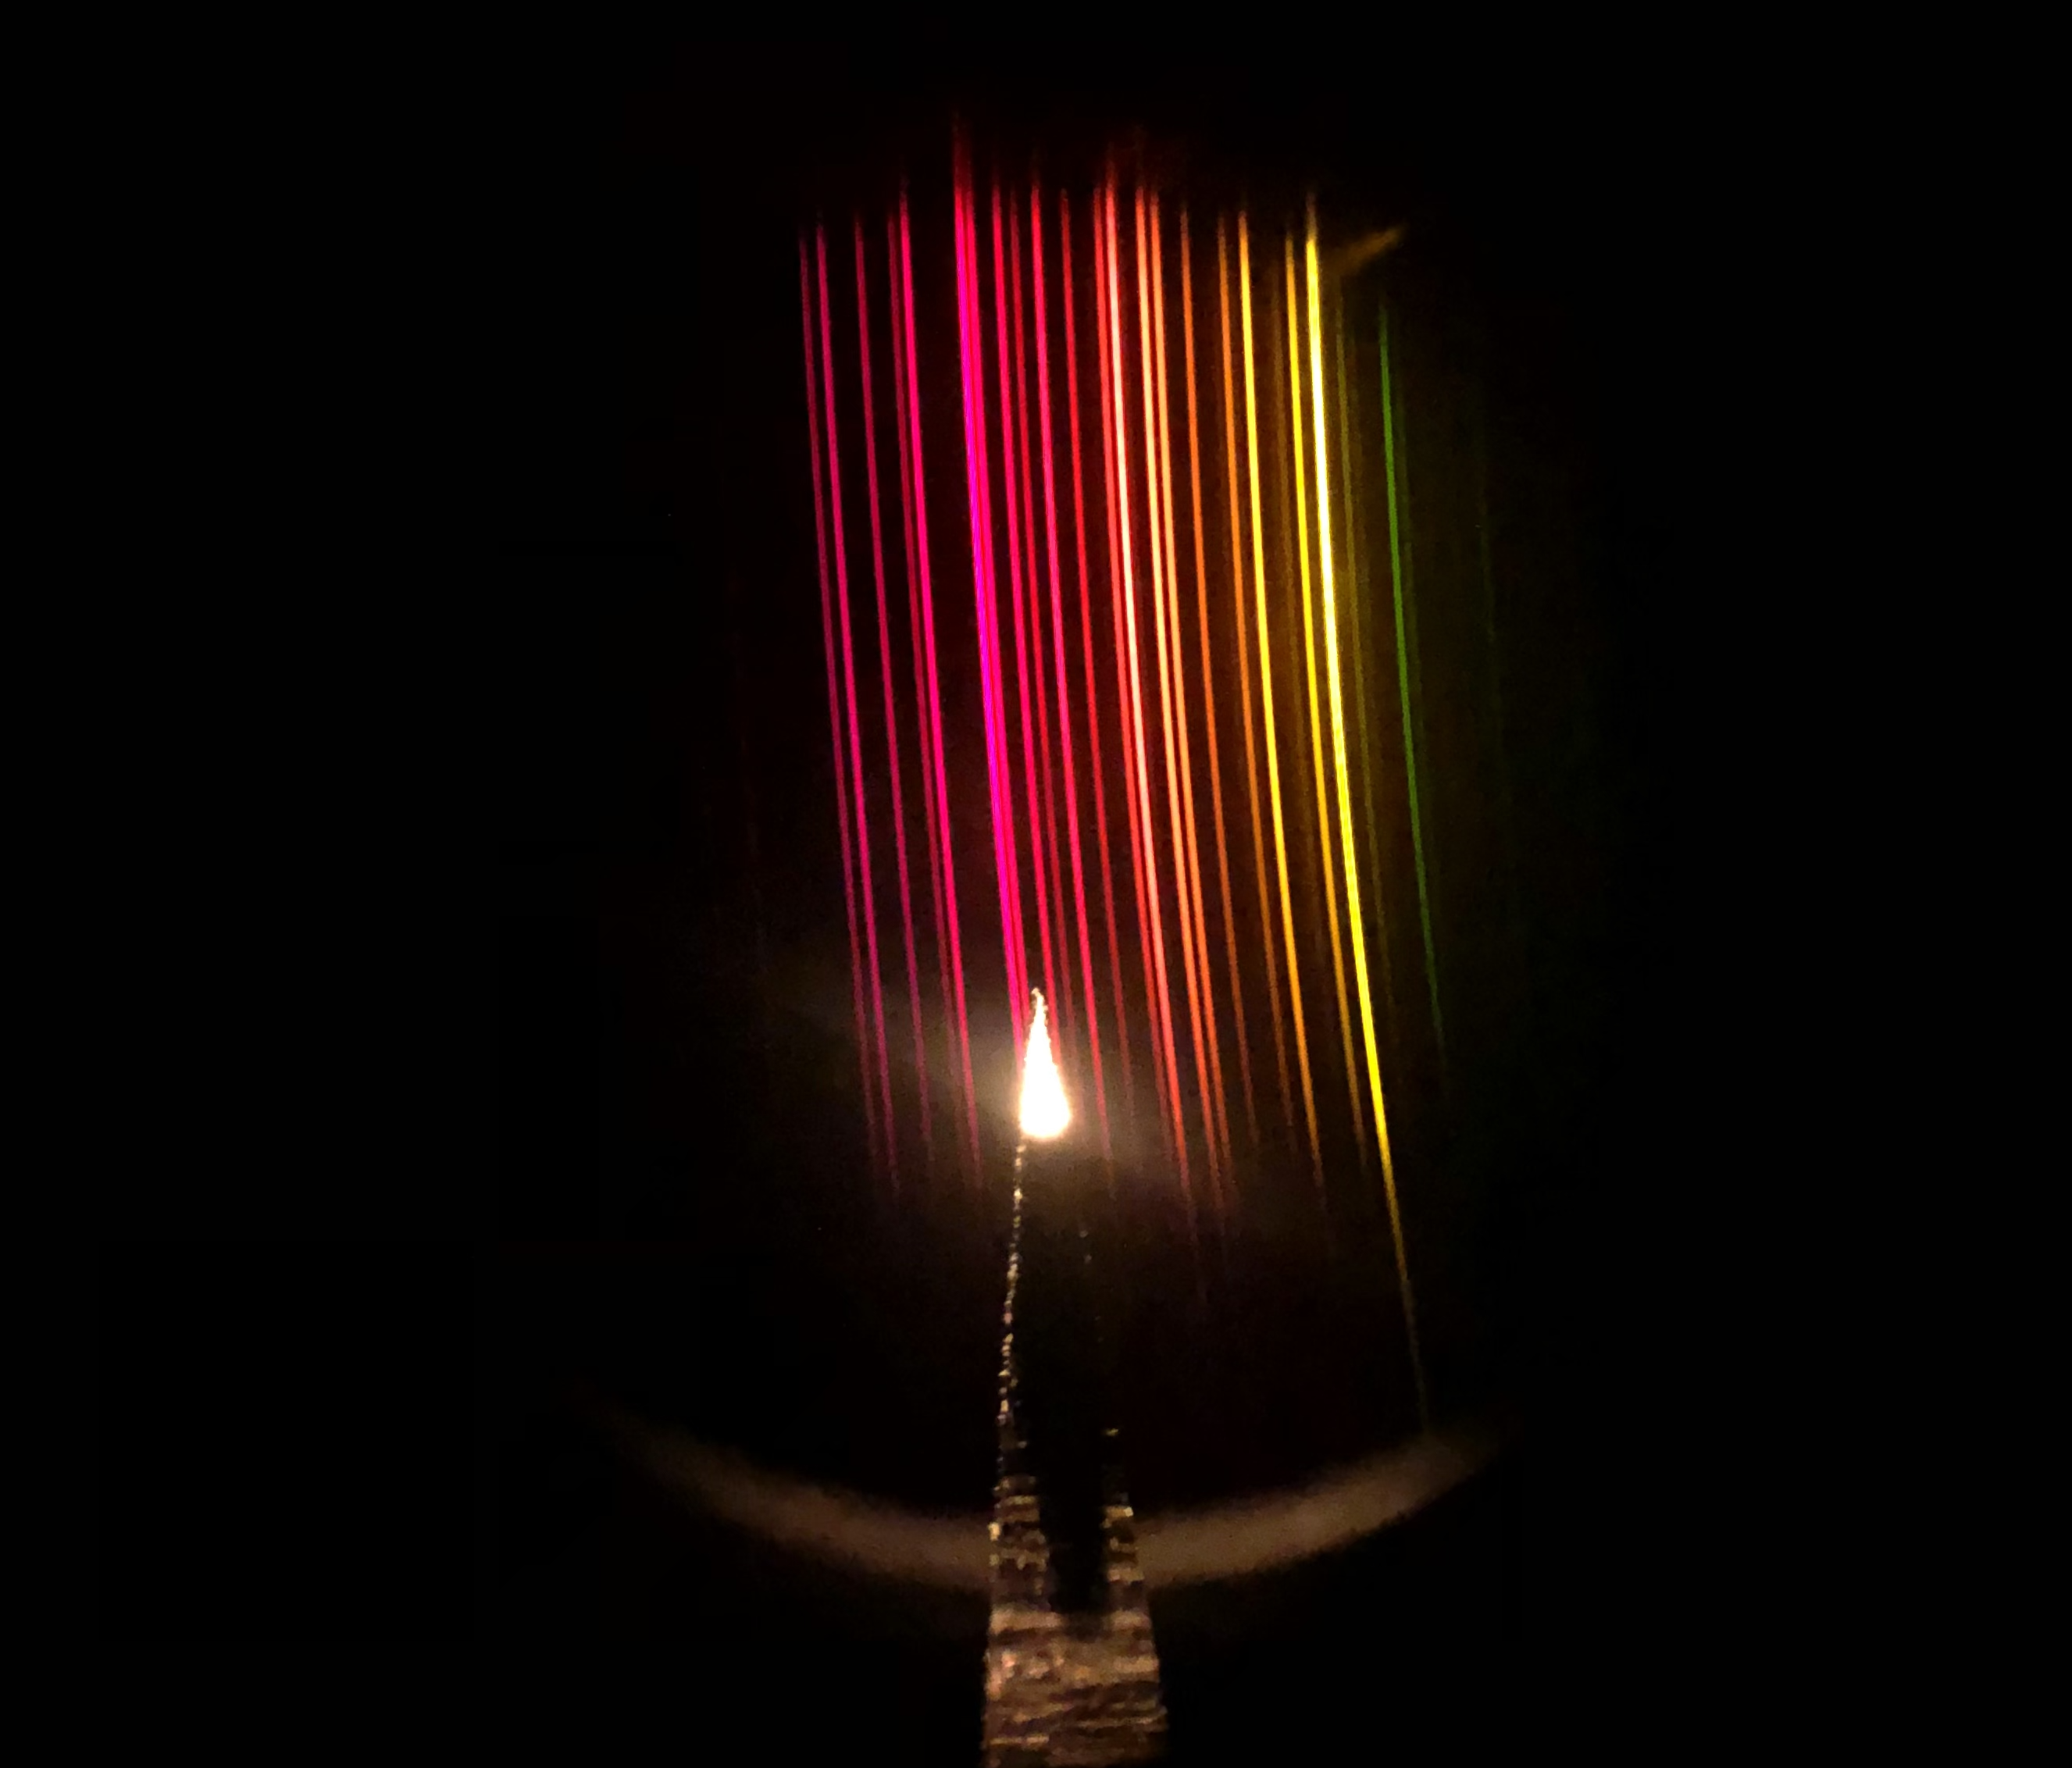
\includegraphics[width = 0.4\linewidth]{Neon_spectre}
 		\includegraphics[width = 0.4\linewidth]{Rtut_spectre}
 		\caption{Наблюдемый спектр испускания водорода}
 	\end{figure}

 	\begin{table}[h!]
 		\centering
 		\caption{таблица градуировки для неона и ртути}
 		\begin{tabular}{|c|c|c|c|c|c|}
 			\hline
 			\multicolumn{6}{|c|}{Неон} \\ \hline
 			n	&	$\lambda$,\AA	&	$\degree$	&	n	&	$\lambda$,\AA 	&	$\degree$	\\ \hline
			1	&	7032	&	2604	&	14	&	6164	&	2303	\\ \hline
			2	&	6929	&	2575	&	15	&	6143	&	2294	\\ \hline
			3	&	6717	&	2511	&	16	&	6096	&	2273	\\ \hline
			4	&	6678	&	2496	&	17	&	6074	&	2262	\\ \hline
			5	&	6599	&	2470	&	18	&	6030	&	2242	\\ \hline
			6	&	6533	&	2446	&	19	&	5976	&	2217	\\ \hline
			7	&	6507	&	2434	&	20	&	5945	&	2202	\\ \hline
			8	&	6402	&	2400	&	21	&	5882	&	2170	\\ \hline
			9	&	6383	&	2388	&	22	&	5852	&	2150	\\ \hline
			10	&	6334	&	2366	&	23	&	5401	&	1887	\\ \hline
			11	&	6305	&	2358	&	24	&	5341	&	1842	\\ \hline
			12	&	6267	&	2344	&	25	&	5331	&	1837	\\ \hline
			13	&	6217	&	2323	&		&		&		\\ \hline
 		\end{tabular}
 		%\caption{таблица градуировки для Ртути}
 		\begin{tabular}{|c|c|c|c|c|c|}
 			\hline
 			\multicolumn{6}{|c|}{Ртуть} \\ \hline
 			n	&	$\lambda$, \AA	&	$\degree$	&	n	&	$\lambda$, \AA	&	$\degree$	\\ \hline
			К1	&	6907	&	2568	&	3	&	5461	&	1926	\\ \hline
			К2	&	6234	&	2325	&	4	&	4916	&	1498	\\ \hline
			1	&	5791	&	2117	&	5	&	4358	&	826	\\ \hline
			2	&	5770	&	2106	&	6	&	4047	&	268	\\ \hline
 		\end{tabular}
 	\end{table}

% 	\begin{table}[h!]
% 		\centering
% 		\caption{таблица градуировки для Ртути}
% 		\begin{tabular}{|c|c|c|c|c|c|}
% 			\hline
% 			n	&	$\lambda$, \AA	&	$\degree$	&	n	&	$\lambda$, \AA	&	$\degree$	\\ \hline
%			К1	&	6907	&	2568	&	3	&	5461	&	1926	\\ \hline
%			К2	&	6234	&	2325	&	4	&	4916	&	1498	\\ \hline
%			1	&	5791	&	2117	&	5	&	4358	&	826	\\ \hline
%			2	&	5770	&	2106	&	6	&	4047	&	268	\\ \hline
% 		\end{tabular}
% 	\end{table}

 	Тогда построим общий градуировочный график 
 	\clearpage
 	\begin{figure}[h!]
 		\centering
 		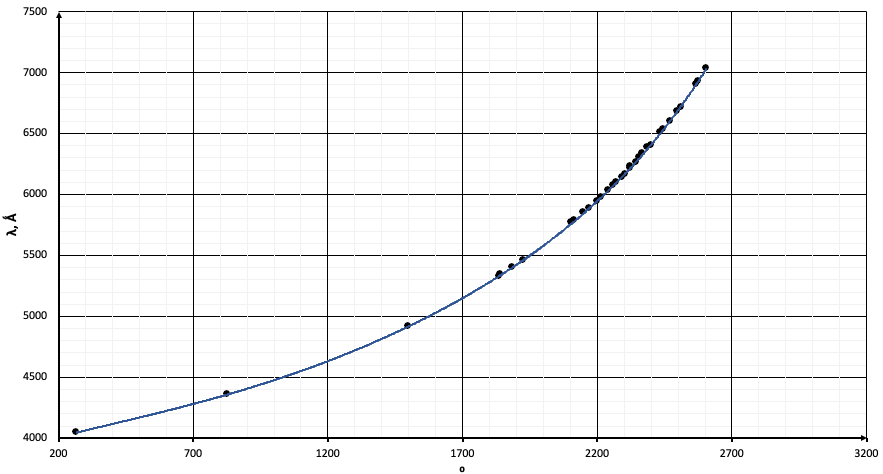
\includegraphics[width = 1.1\linewidth]{graduate}
 		\caption{Градуировочный график}
 	\end{figure}
 	
 	\item Узнаем положение линий $H_\alpha, H_\beta, H_\gamma, H_\delta$ для водородной лампы.
 	\begin{table}[h!]
 		\centering
 		\caption{положение линий $H_\alpha, H_\beta, H_\gamma, H_\delta$ и постоянная Ридберга}
 		\begin{tabular}{|c|c|c|c|}
 			\hline
 			$H$& $\lambda,$\AA&$\degree$ & $R, 10^6м^{-1}$\\ \hline
 			$H_\alpha$ & 6520 & 2454& 1,103 \\ \hline
 			$H_\beta$ & 4980 & 1446 & 1,071\\ \hline
 			$H_\gamma$ & 4370 & 798 & 1,091\\ \hline
 			$H_\delta$ & 4110 & 372 & 1,095\\ \hline
  		\end{tabular}
 		
 	\end{table}
 	\\
 	Тогда $R_{ср} = 1,090 \pm 0,02\cdot 10^6м^{-1}$ 
 \end{enumerate}
 \clearpage
 \subsection*{Б) Изучение молекулярного спектра йода}
 \begin{enumerate}
 	\item Для йода наблюдаем такой спектр
 	
% 	\begin{minipage}{0.47\linewidth}
% 		
% 	 	\centering
% 	 	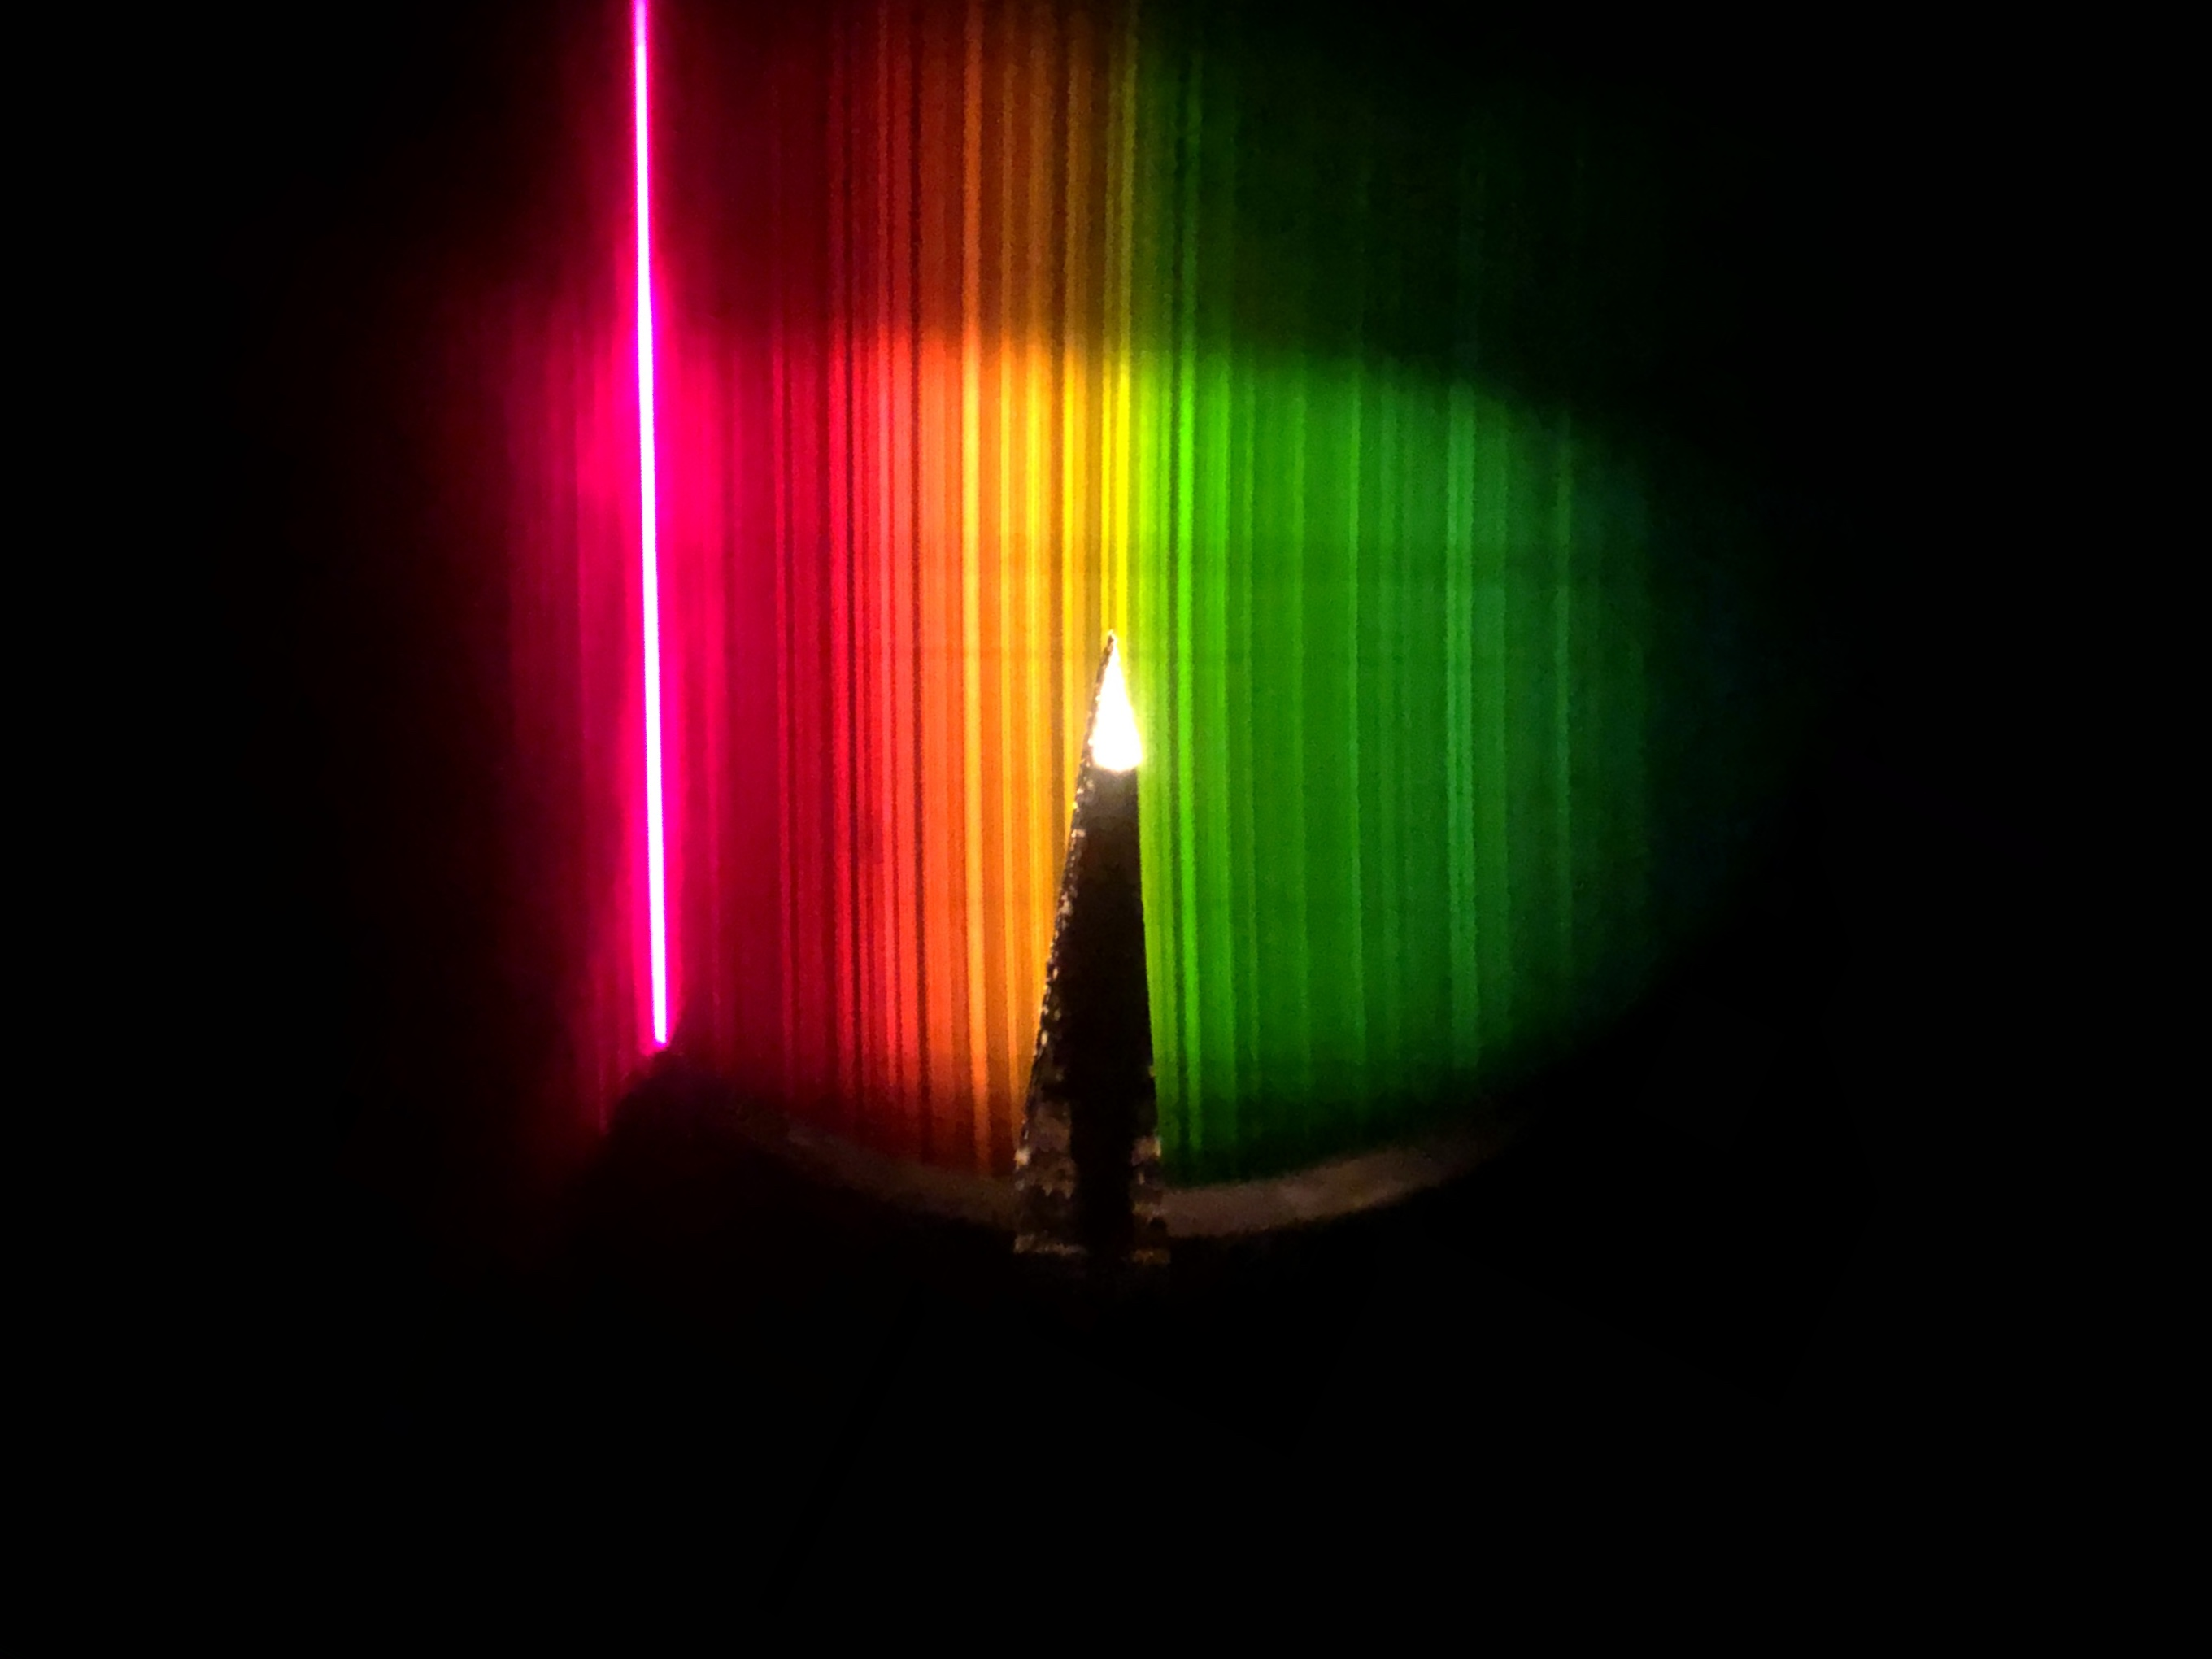
\includegraphics[width = \linewidth]{I_spectre_1}
% 	 	 
% 	\end{minipage}
%	\begin{minipage}{0.47\linewidth}
% 		\centering
% 	 	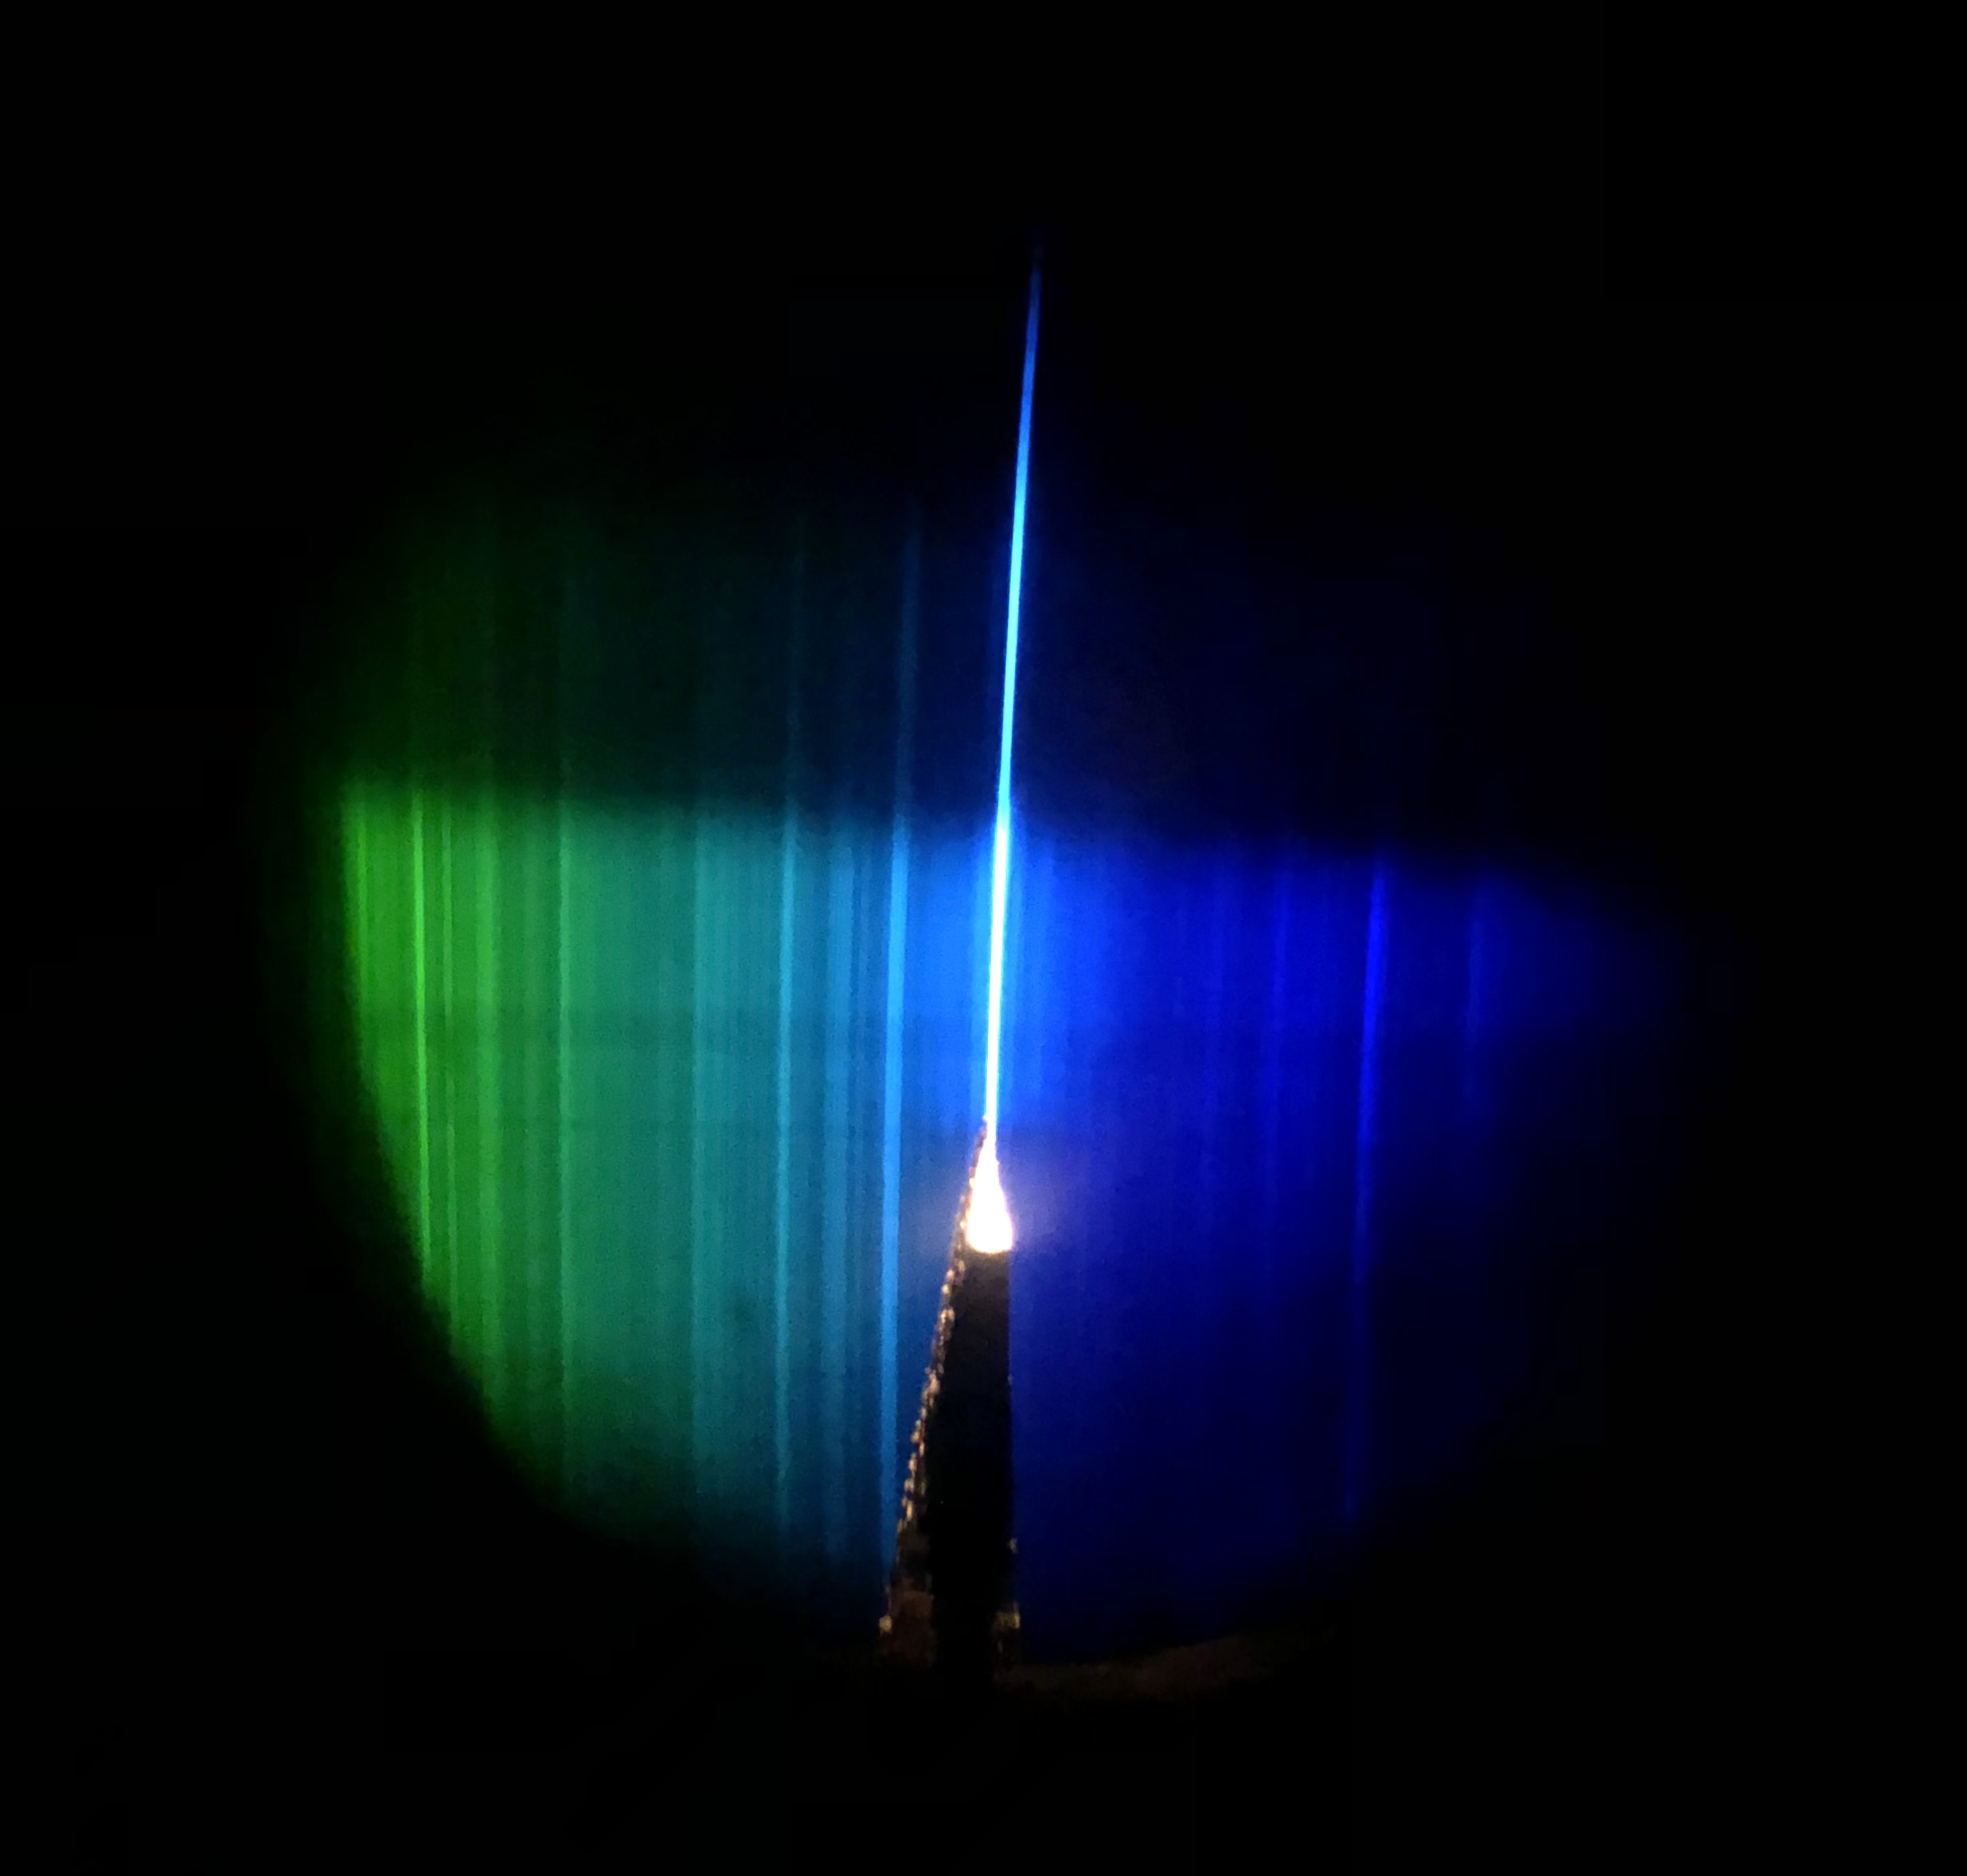
\includegraphics[width = \linewidth]{I_spectre_2}
% 	 	
% 	\end{minipage}
 		
 	\begin{figure}[h!]
 		\centering
 		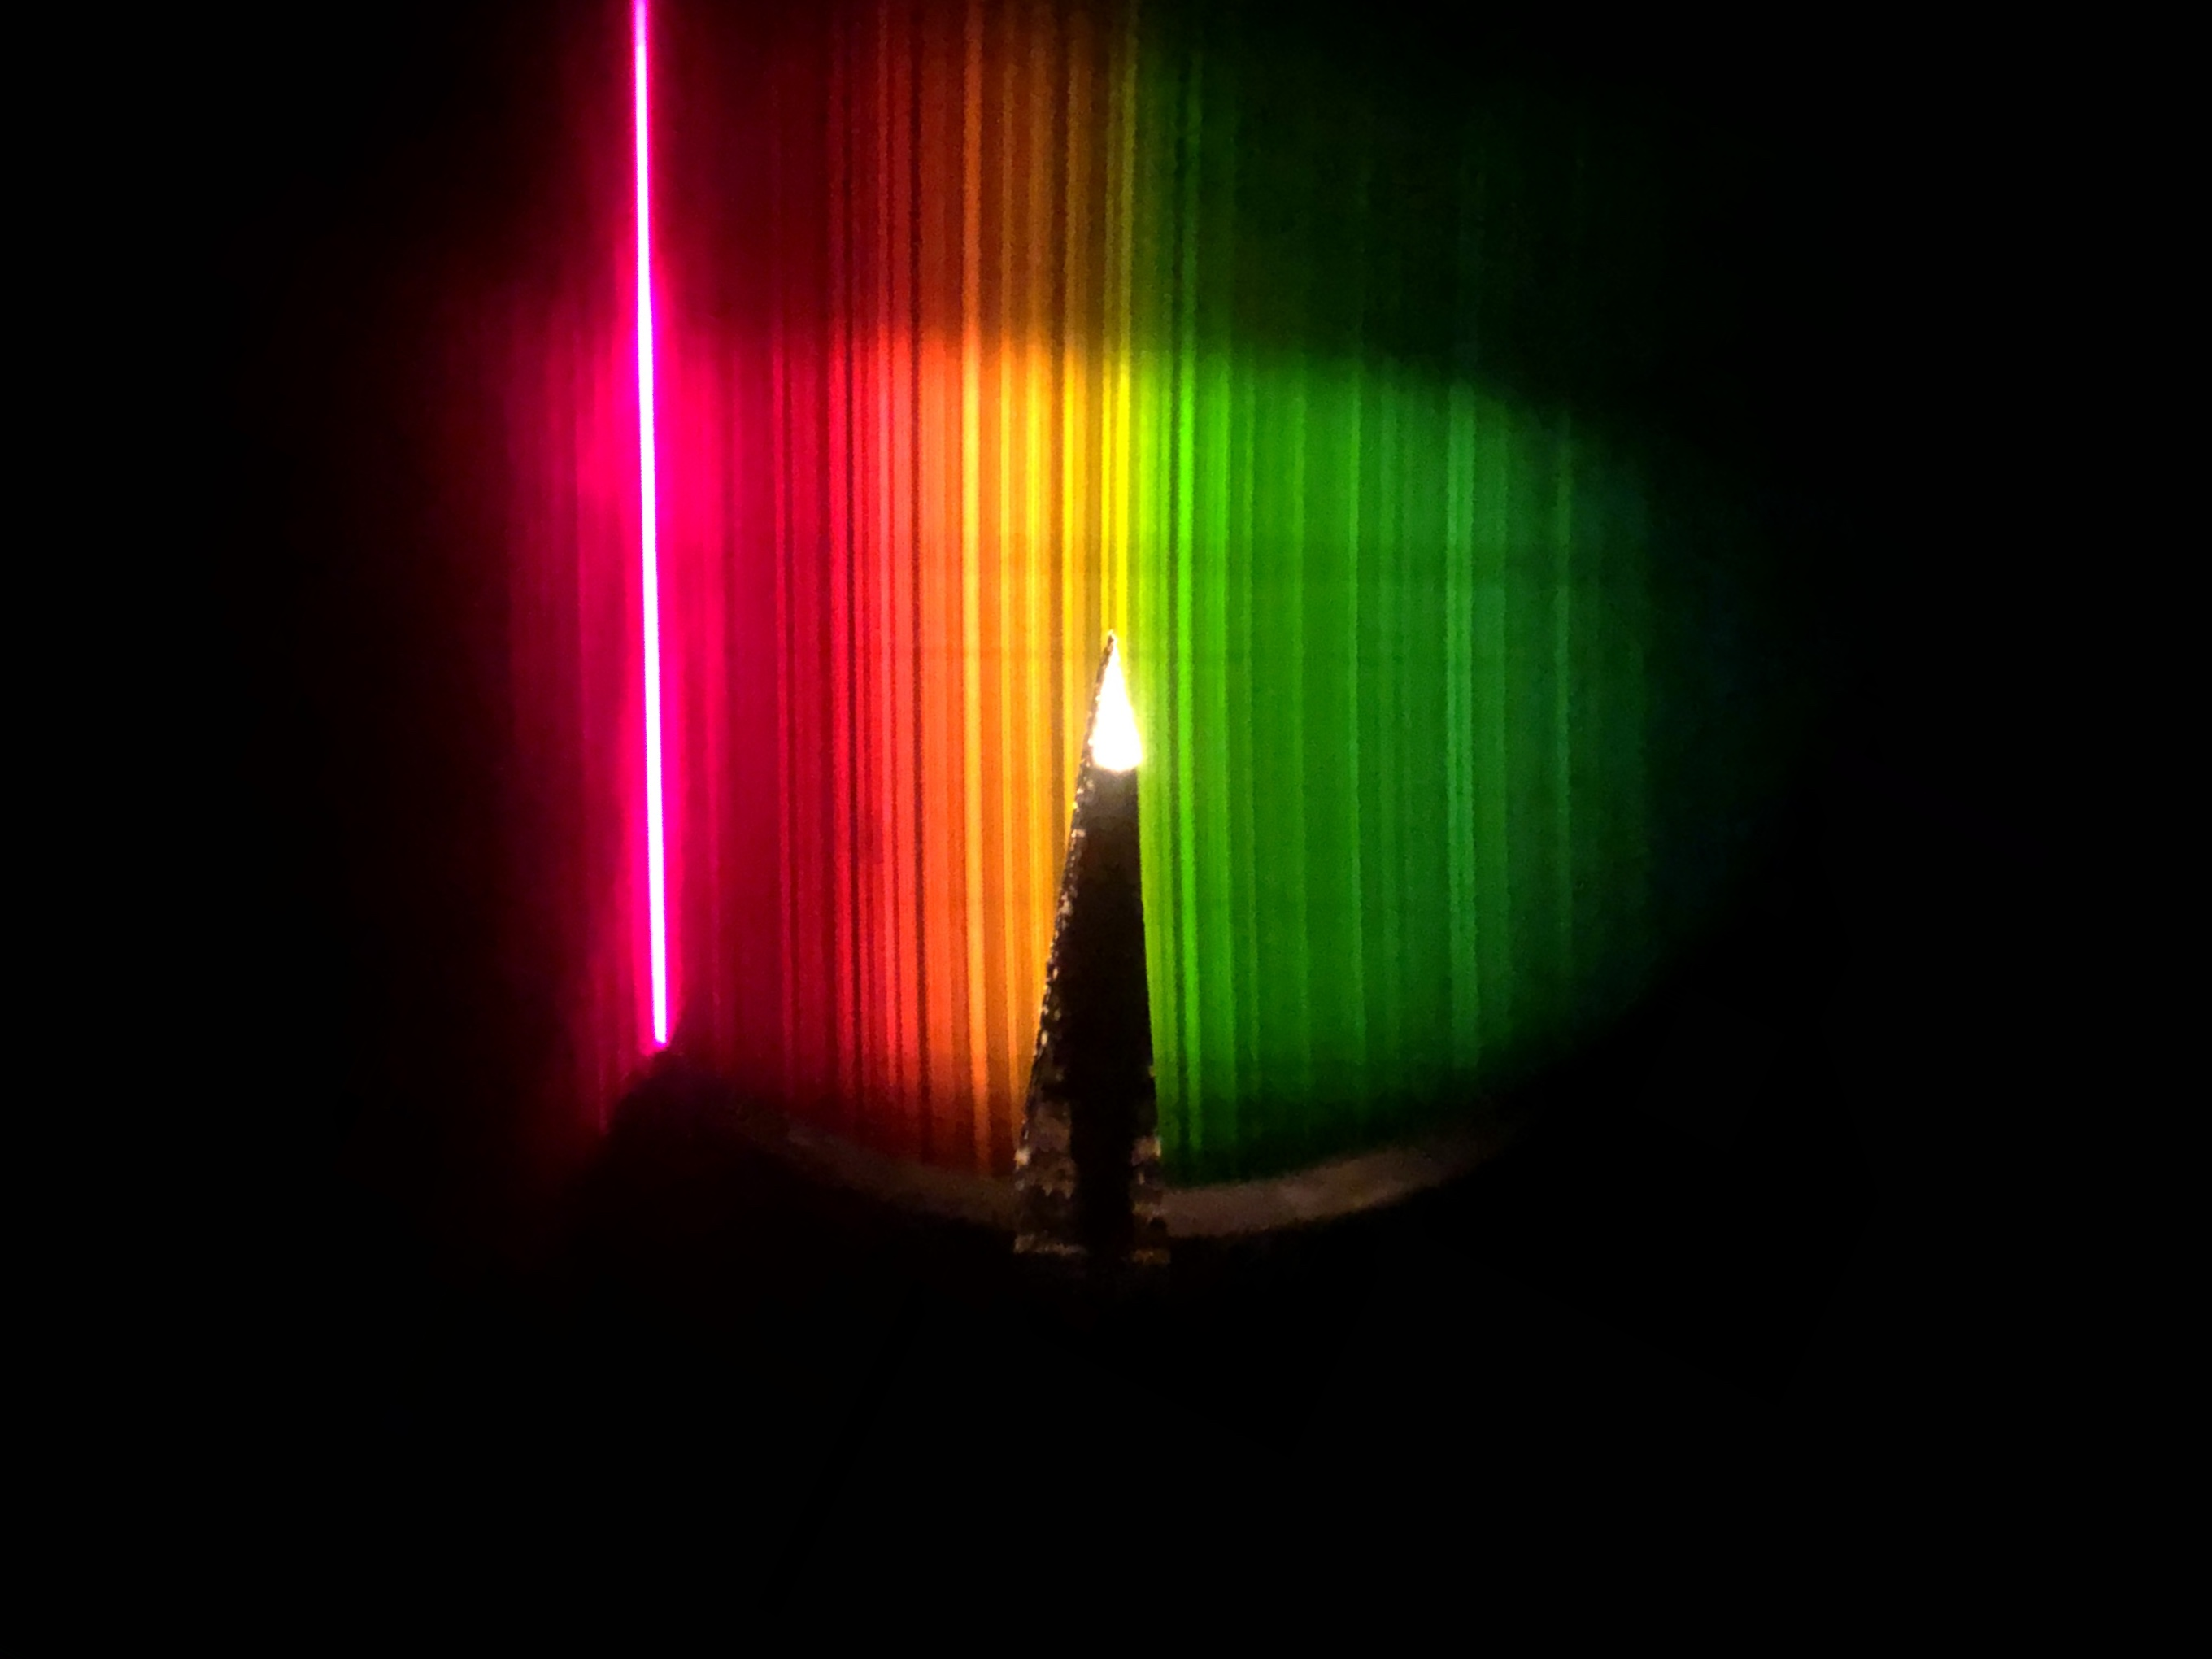
\includegraphics[width = 0.4\linewidth]{I_spectre_1}
 		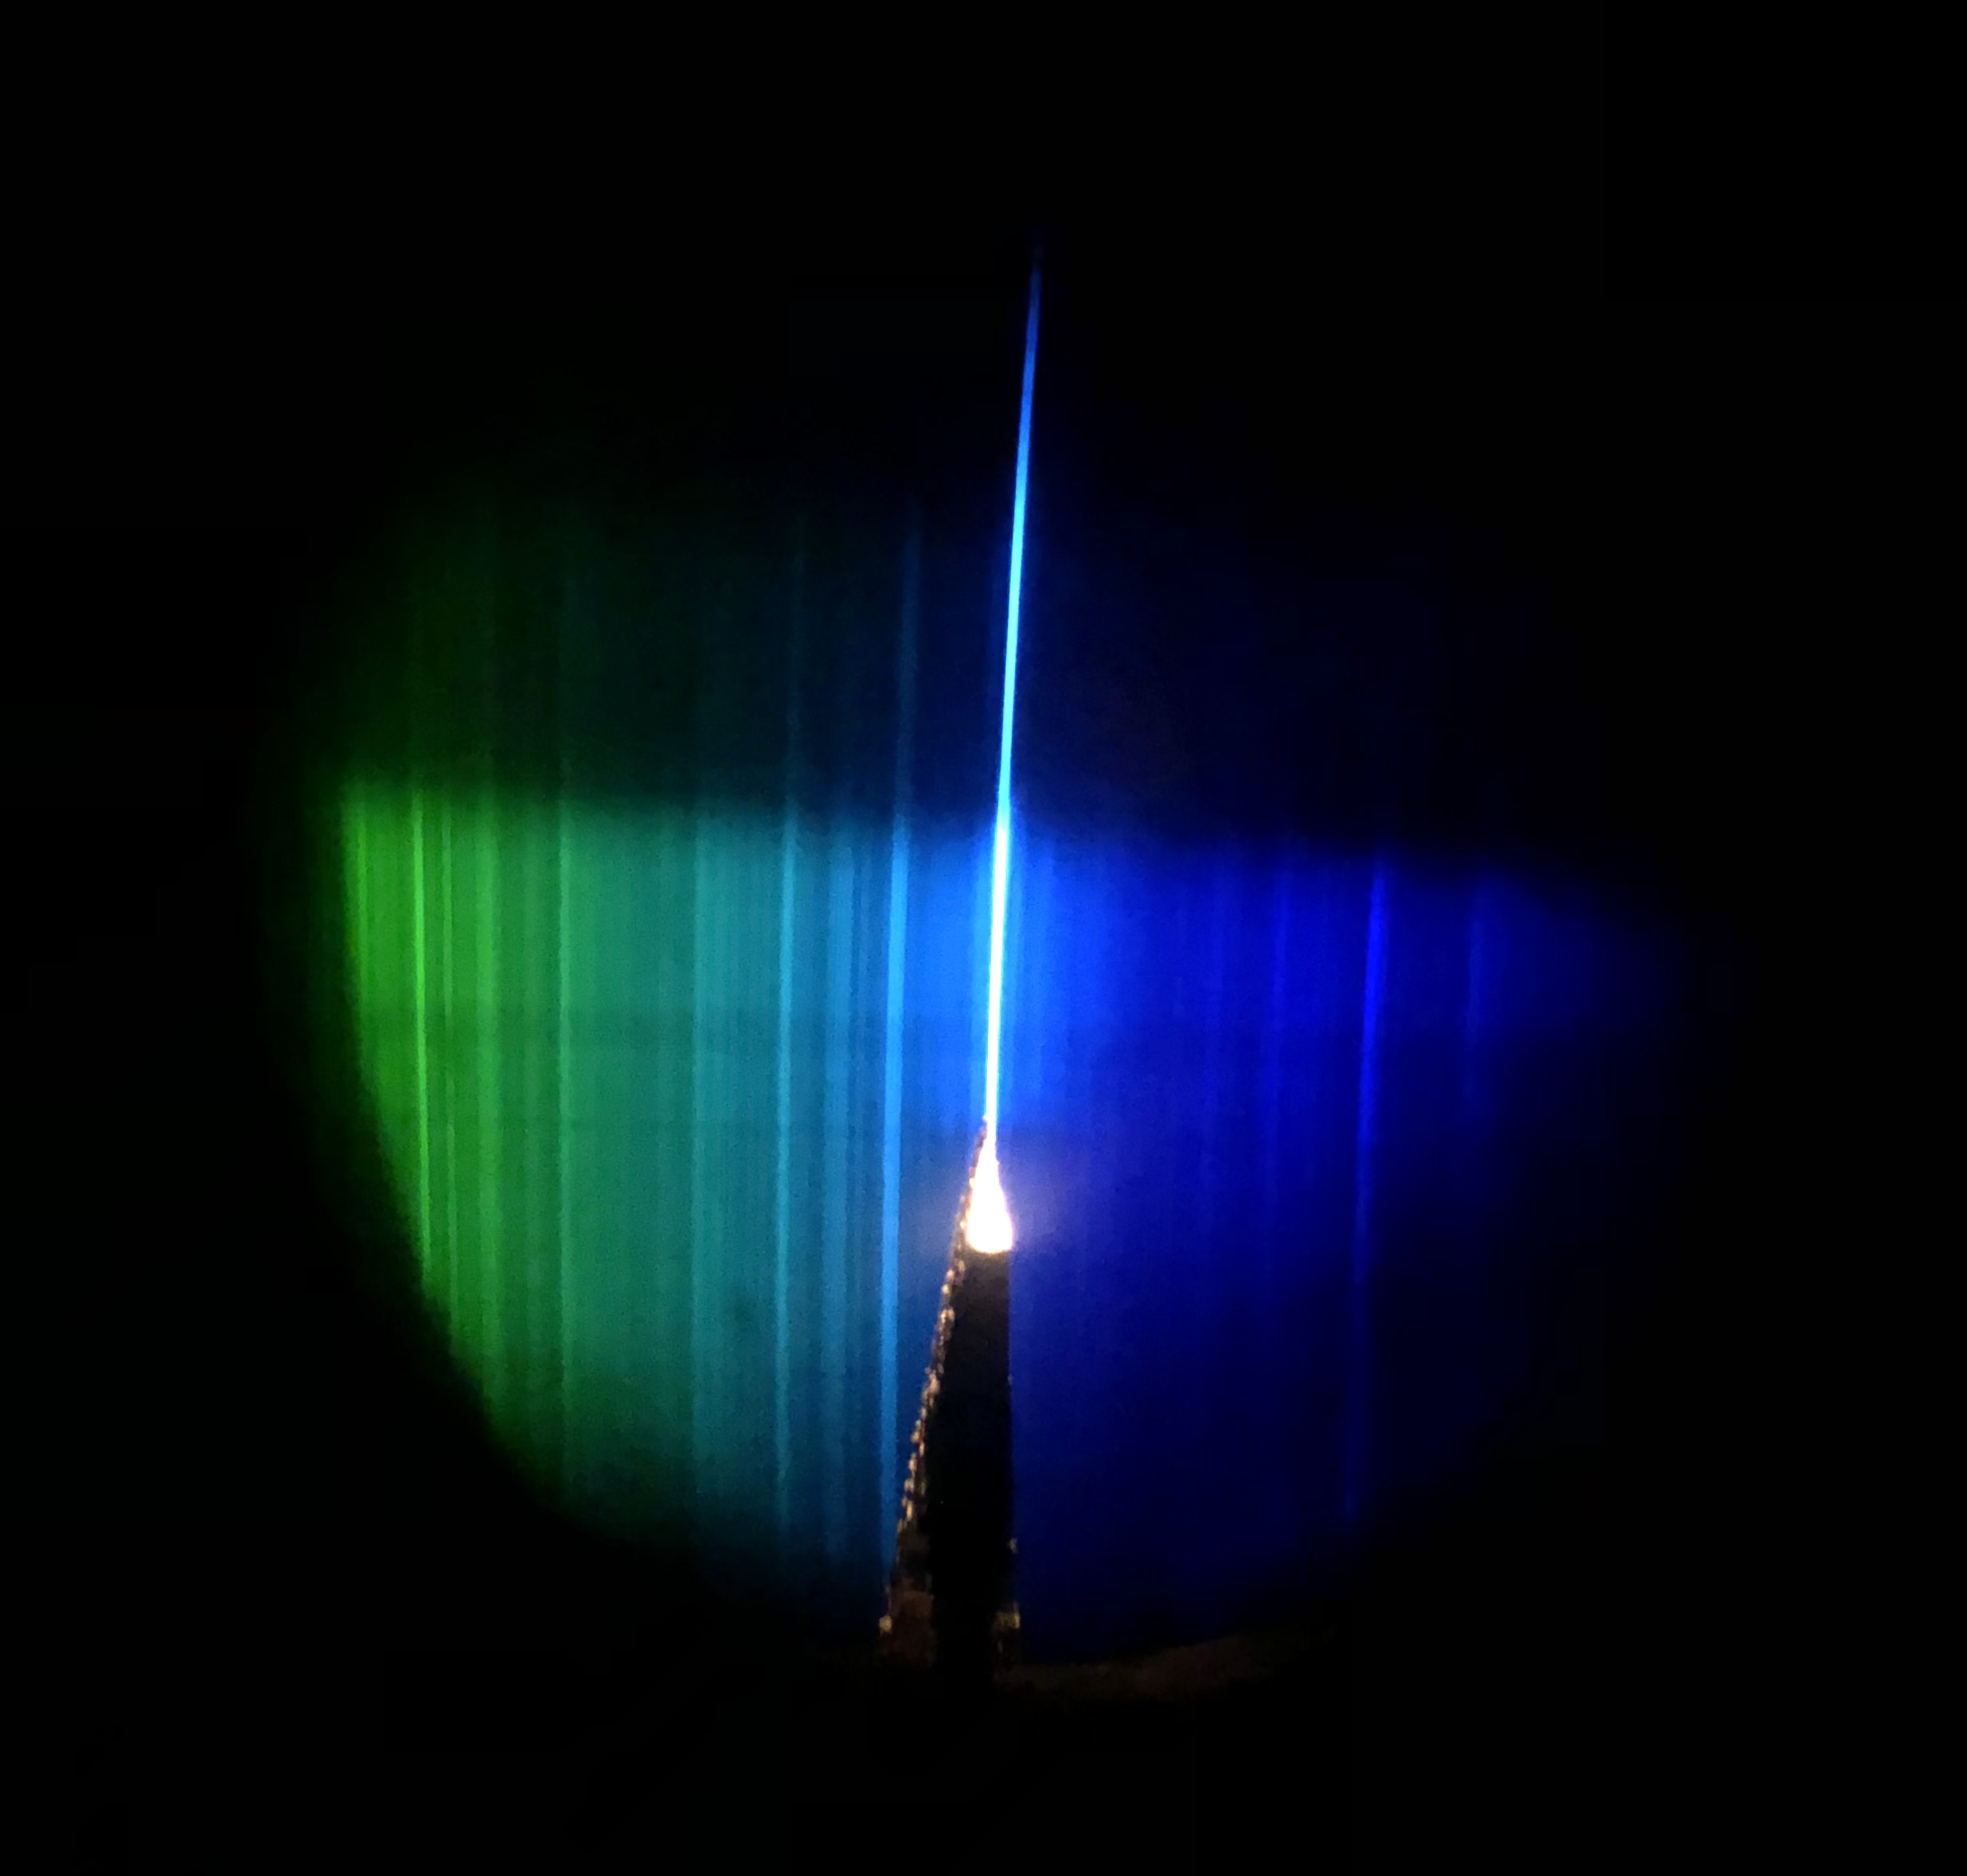
\includegraphics[width = 0.4\linewidth]{I_spectre_2}
 		\caption{Наблюдаемый спектр поглощения йода}
 	\end{figure}
 		\item Найдем координаты линий $n_{1,0}, n_{1,5}, n_{гр}$
 		\begin{table}[h!]
 			\centering
 			\caption{Координаты линий спектра йода}
 			\begin{tabular}{|c|c|c|}
 			\hline
 				Линия & $\degree$& $\lambda,$\AA \\ \hline
 				$n_{1,0}$& 2234 & 6140 \\ \hline
 				$n_{1,5}$& 2143 & 5980 \\ \hline
 				$n_{гр}$&1648&1650 \\ \hline
 			\end{tabular}
 		\end{table}
 	\item Вычислим в электрон-вольтах энергию колебательного кванта возбужденного состояния молекулы йода: $h\upnu_2 = (h\upnu_{1,5}-h\upnu_{1,0})/5 = 0,00103 \ эВ$ 
 	\item Пользуясь полученными данными, а также данные о том, что $h\upnu_1 = 0,027 \ эВ$ - энергияколебательного кванта основного состояния и E = $0,94 \ эВ$ - энергия возбждения атома, вычислим:
		\begin{itemize}
			\item Энергию электронного перехода $h\upnu_{эл} = 1,68 \ эВ$
			\item Энергию диссоциации молекулы в основном состоянии $D_1$ =  1,43 эВ
			\item Энергию диссоциции молекулы в возбужденном состоянии $D_2 = 0,69$ эВ
		\end{itemize} 


 \end{enumerate}
 % section ход_работы (end)
 \section{Итоговые результаты}
 Из первого эксперимента: $R = (1,090 \pm 0.020)\cdot 10^6м^{-1}$
 Из второго эксперимента: $D_1 = 1,43\ эВ, h\upnu_{эл} = 1,68эВ, D_2 = 0,69эВ $
 \section{Вывод}
 Мы изучили спектры в оптических спектрах водорода и йода, экспериментально проверили справедливость формулы Бальмера и нашли постоянную Ридберга, которая в пределах погрешности совпадает с табличной ($ R = 109 677,6 \ см^{-1} $), и оценили энергии квантов возбужденного состояния молекулы, энергию диссоциации частиц и энергию электронного перехода.
	
 % section section_name (end)
\end{document}
